Our approach touches several research areas, including computation and visualization of protein cavities and their surfaces. 
Further we focus on the real-time visualization of surfaces and their transparency which is achieved by using the order-independent transparency approach. 
%Thus in this section we describe the existing techniques related to these topics.

\subsection{Extraction and Visualization of Molecular Surfaces}
There are several types of molecular surface representation proposed in the literature~\cite{STAR2015}. 
%One of the most recently defined surfaces is the ligand-excluded surface proposed by Lindow et al.~\cite{Lindow2014} which takes into account the full geometry of the ligand interacting with the protein.
Regarding the cavity analysis, the solvent-excluded surface (SES) is the most commonly used representation preferred also by the domain experts.
This representation allows us to directly asses whether a ligand, approximated by a sphere of a given radius, can penetrate through the molecular surface. 
The field of geometrical analysis of molecular structures focusing on the detection and further exploration of the void space is very vast and, therefore, we relate only to the techniques that we consider to be relevant and close to our work. 

%The molecular surface represents one of the most significant studied features thus many solutions were published.
In 1983, Connolly proposed an analytical approach for construction of the SES representation~\cite{connolly1983analytical}.
In 1996, Sanner et al.~\cite{Sanner1996} introduced the reduced surface algorithm to construct SES. In the same year, Totrov and Abagyan~\cite{totrov1996contour} introduced the contour-buildup algorithm to create SES representation. The algorithm is based on the sequential buildup of multi-arc contours. 
One of the advantages of this approach is its spatial localization meaning that it is applicable to partial molecular surfaces.
In 1995, Edelsbrunner et al.~\cite{Edelsbrunner1995} proposed to exploit alpha shapes to detect and measure the voids in proteins.
Another approach, linearly scalable algorithm for computation of smooth molecular surfaces was then presented by Varshney et al.~\cite{Varshney1994}.

One of the significant improvements of the SES computation was published by Parulek and Viola~\cite{parulek2012implicit}.
Their approach does not require any precomputation. 
It is based on the theory of implicit surfaces where the value of the implicit function helps to determine the inner and outer points with respect to the surface.
The implicit function is composed of three types of patches from which the SES is constructed.

However, none of these solutions dealt with molecular dynamics. 
Krone et al.~\cite{krone2009interactive} presented their approach to the visualization of the SES using GPU ray-casting technique which allowed to achieve interactive frame rates. 
Another approach by Lindow et al.~\cite{lindow2010accelerated} even accelerated the construction of the SES by scaling the parallel contour-buildup algorithm to more CPU cores and using boundary quadrangles as rasterization primitives.
Moreover, Krone et al.~\cite{krone2011parallel} proposed a parallel version of the contour-buildup algorithm for GPUs that performed better for larger structures.
In our approach, we further extend it so that the computed SES can be rendered using correct transparency.

Similarly, the analytical approaches are applicable to the protein inner voids. 
We focus only on the analytical computation and visualization of cavities which can contain a potential protein binding site.
Parulek et al.~\cite{parulek2013visual} presented their approach to the computation and visual analysis of cavities in simulations of molecular dynamics.
The computation is based on implicit function. 
The subsequent exploration is supported by graph based visualizations.
Another approach to the visual analysis of dynamic protein cavities and binding sites was proposed by Krone et al.~\cite{Krone2014}.
Their system combines semi-transparent surface visualizations with sequence diagrams and relational graphs to communicate different properties of detected cavities.
Lindow et al.~\cite{Lindow2013} presented an alternative approach to the exploration of the time-dependent changes of a cavity. 
To avoid the animation of the traced cavity, they visualize the dynamics of the cavity as a compact representation in a single image, color coded according to time. 

\begin{figure*}[tb]
  \centering
  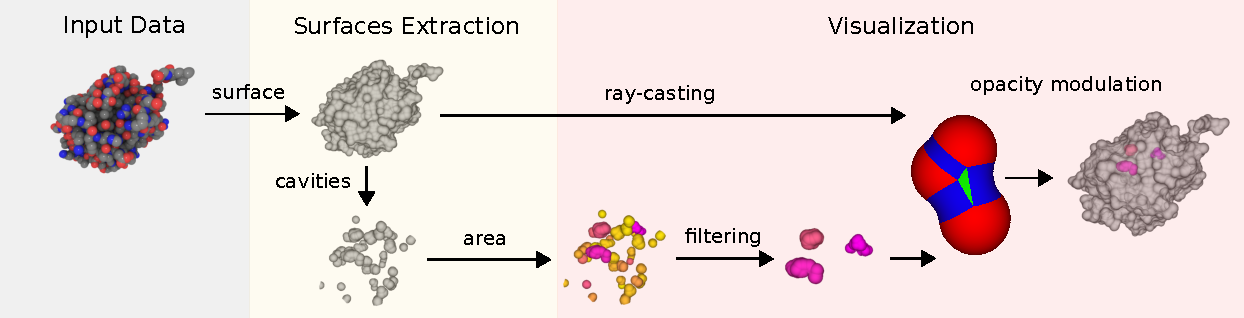
\includegraphics[width=\textwidth]{image/overview_final.pdf}
  \caption{Illustration of the visualization pipeline. The input data (Sec.~\ref{ch:overview}) contains snapshots of MD trajectories which are processed to construct the molecular surface and cavities (Sec.~\ref{ch:feature}). Then, the surface areas of cavities are estimated (Sec.~\ref{sec:area}), which are used as the color codes, ranging from yellow (smallest) to magenta (largest). These areas serve for filtering out of too small cavities. Finally, the surface elements are ray-cast (Sec.~\ref{sec:spherical-patches}) to compose the surface fragments used in the final stage to visualize the surfaces transparently via a user-defined opacity modulation (Sec.~\ref{sec:opacity}).}
	\label{fig:overview}
\end{figure*}

\subsection{Visualization of Surface Features}
There are also several visualization techniques enhancing the visibility of molecular surface features located inside the molecule. The main source of these techniques is described in the computer graphics literature. Bair and House~\cite{Bair2007} presented an approach for visualization of layered surfaces, which uses grid-based surface textures. Their experiments focus on the perception of textured surfaces and the best configuration of the textures. 
Other illustrative techniques presented by Tarini et al.~\cite{Tarini2006} and Lawonn et al.~\cite{Lawonn2014} represent alternatives to the visualization of the shape of molecular surfaces. 
These techniques are based on ambient occlusion or its combination with line integral convolution and were not designed to show more layered surfaces.

One of the most popular techniques for rendering transparent objects is the order-independent transparency (OIT) which does not require the geometry to be sorted.
Here the traditional approaches are Virtual Pixel Maps (know also as Depth Peeling) \cite{mammen1989transparency} or A-buffer \cite{carpenter1984abuffer}.
Thanks to the performance of the current hardware these methods can be successfully adopted to large and dynamic scenes.
The Virtual Pixel Maps technique is based on the idea of sorting at the pixel level and accumulating the transparency effect on a multipass basis. 
%The A-buffer uses the Fourier window which in general helps to resolve the visibility problem among an arbitrary collection of opaque, transparent, and intersecting objects.

While the algorithms for rendering of correctly transparent objects in real-time have emerged already in the previous decade \cite{everitt2001interactive}, new approaches removing the limitations of these methods are still emerging.
Bavoil et al.~\cite{bavoil2008order} introduced the peeling of two depth layers in one rendering pass, thus halving the number of rendering passes performed by the original Depth Peeling approach \cite{everitt2001interactive}. However, in our case performing more rendering passes would become a bottleneck because of our ray-tracing approach to the surface rendering.
Thus, techniques based on the A-buffer suit our technique since they enable to render the entire scene in one pass.
When using single pass rendering, it is necessary to store all participating or at least all important fragments into a data structure for later composition.
The first approach storing the participating fragments was introduced by Yang et al.~\cite{yang2010real}. Salvi et al.~\cite{salvi2011adaptive} presented another approach, wherein it is required only to store the important fragments.
%The cost of single pass rendering is the necessity of storing all participating \cite{yang2010real} or all important \cite{salvi2011adaptive} fragments into a data structure for later composition.
Storing the fragments leads to an unbounded requirement on the memory size that was addressed by Maule et al.~\cite{maule2012memory} or Vasilakis et al.~\cite{vasilakis2015k+buffer}.
Some of the existing techniques aim to decrease both time and memory complexity.
McGuire and Bavoil~\cite{mcguire2013weighted} employ the idea of partial coverage to reach this goal, whereas Enderton et al.~\cite{enderton2011stochastic} introduce stochastic transparency for the same purpose. 
Here each fragment of the transparent geometry covers a random subset of pixel samples of a size proportional to alpha. 
After averaging, the results possess correct alpha-blended colors. 

Applying the aforementioned OIT approaches to molecular surfaces is straightforward since they are represented as meshes.
For analytic surfaces, Kauker et al.~\cite{kauker2013rendering} proposed to store lists (or arrays) of all fragments produced by the basic shapes for later processing using CSG operations.
In our technique, we avoid storing and subsequent sorting of a high number of fragments by ray-casting only those fragments that belong to the molecular surface.
For enhancing the understanding of the interior of the molecular structure, we took inspiration from the technique presented by Borland~\cite{borland2011ambient}. 
The technique, called ambient occlusion opacity mapping, enables to determine a variable opacity at each point on the molecular surface.
In consequence, the interior structures can be more opaque than the outer structures, i.e., molecular surface.

%There are also several alternatives for visualization of molecular surfaces which do not utilize transparency for conveying the same or similar information as we are aiming to show.
%Bair and House~\cite{Bair2007} presented their approach to the visualization of layered surfaces which uses grid-based surface textures.
%Their experiments focused on the perception of textured surfaces and the best configuration of the textures. 
%Other illustrative techniques presented Tarini et al.~\cite{Tarini2006} and Lawonn et al.~\cite{Lawonn2014} represent alternatives to the visualization of the shape of molecular surfaces. 
%However, these techniques, based on ambient occlusion or its combination with line integral convolution, were not designed to show more layered surfaces.



%\subsection{Ambient Occlusion}
%Ambient occlusion is one of the most popular techniques for enhancement of the depth perception in molecular visualization.
%Tarini et al.~\cite{tarini2006ambient} as first used this technique for real-time molecular visualization.
%As this technique is computationally very demanding, several solutions focusing on this limitation appeared.
%Grottel et al.~\cite{grottel2012object} presented their method reaching interactive frame rates for large and dynamic data sets. 
%Recently, their approach was extended by~\cite{staib2015ambient}.
%This method is applicable to transparent particles as well.
%\textcolor{red}{TODO move to Visualization or remove completely:

%\begin{itemize}
%  \item \textcolor{red}{Performance drop of SES rendering on newer hardware (GF 680 GTX) --- we can perform better. We contacted authors, they do not know exactly why, they think it is change in the internal architecture between Fermi and Kepler (AJ)}
%  \item \textcolor{red}{Slow rendering of SAS. Too many layers in pixels --- we can do better by surface layers detection (AJ)}
%\end{itemize}

%\textcolor{red}{There are more solutions taken from computer graphics; e.g., OIT (JP)}

%Such binding site can be located inside a cavity or a tunnel, while the molecular surface might contain tens of cavities per single simulation time step. 


